\begin{refsection}

\chapter{The Majorise-Minimise Meta-Algorithm}
\label{chap:perturb}

\begin{tcolorbox}
This chapter introduces several classic iterative optimisation methods. The derivations, while themselves not novel, are put on common footing by showing how each corresponds to a form of perturbation analysis.
\end{tcolorbox}

This chapter surveys classic techniques for formally deriving gradient-based optimisation methods. The survey covers first-order methods---such as \textit{gradient descent} and \textit{mirror descent}---as well as second-order methods---such as the \textit{cubic regularised} version of  \textit{Newton's method}. These varied techniques are put on a consistent theoretical footing by showing that one step of each method may be viewed as the minimisation of a particular local description of the loss function. In each case, this local description takes the form of a \textit{perturbation bound} on the error of a \textit{truncated perturbation expansion} of the loss. Such bounds, known as \textit{majorisations}, assess the region within which the perturbation expansion can be trusted.

The optimisation methods described in this chapter make use of perturbation expansions and bounds related to the Taylor series expansion of the loss function $\el$ in the weight space $\mathcal{W}$ of the optimisation problem. As such, they may construct a perturbation $\Delta w\in\mathcal{W}$ to the weights $w\in\mathcal{W}$ by considering any of the following information:
\begin{enumerate}
    \item \textit{First-order information}: The gradient $\nabla_w \el(w)$ of the loss function.
    \item \textit{Second-order information}: The Hessian $\nabla_w^2 \el(w)$ of the loss function.
    \item \textit{Trust regions}: Bounds on the accuracy of the above information.
\end{enumerate}

In contrast to the techniques considered in this chapter, Chapter \ref{chap:maj-min} deals more closely with neural networks. There the loss $\el$ depends on the weights $w\in\mathcal{W}$ indirectly via the network architecture $f(\cdot;w):\mathcal{X}\to\mathcal{Y}$, and it will help to model this dependence. But in this chapter, the loss function will be viewed as a straightforward function of the weights---formally, the loss $\el : \mathcal{W} \to \R$.

\section{Perturbation analysis: Expansions and bounds}
This section introduces the general ideas of perturbation analysis. Section \ref{sec:mm} will show how these ideas may be used to solve optimisation problems.

\subsection{Perturbation expansions}
The simplest example of a perturbation expansion is a straightforward Taylor series. Provided a function $g:\R\to\R$ is analytic, it may be expanded about a point $x\in\R$ as a Taylor series in powers of some small perturbation $\delta x\in\R$:
\begin{equation}\label{eq:taylor}
    g(x+\delta x) = g(x) + \frac{\partial g}{\partial x}\cdot\delta x + \frac{1}{2} \frac{\partial^2 g}{\partial x^2}\cdot\delta x^2 + ...
\end{equation}

A \textit{truncated} perturbation expansion refers to cutting off this series at some order. For instance, truncating Equation \ref{eq:taylor} yields:
\begin{equation}\label{eq:p-expand}
    g^{(2)}(x+\delta x) \coloneqq g(x) + \frac{\partial g}{\partial x}\cdot\delta x + \frac{1}{2} \frac{\partial^2 g}{\partial x^2}\cdot\delta x^2,
\end{equation}
where the superscript $(2)$ indicates a second-order truncation.

\subsection{Perturbation bounds}
While the truncated perturbation expansion in Equation \ref{eq:p-expand} is accurate for sufficiently small $\delta x$, the error in this approximation is unknown without computing the truncated part of the series. A \textit{perturbation bound} deals with this issue by bounding the error in a truncated perturbation expansion. For example, if one can derive a function $h(x,\delta x)$ such that:
\begin{equation}\label{eq:p-bound}
    \left|g(x+\delta x) - g^{(2)}(x+\delta x)\right| \leq h(x,\delta x),
\end{equation}
then Inequality \ref{eq:p-bound} would constitute a perturbation bound. For the perturbation bound to be useful, one aspires to finding a bounding function $h(\cdot,\cdot)$ that:
\begin{enumerate}
    \item provides a reasonably tight bound on the error in the truncated series.
    \item is much cheaper to compute than the omitted terms in the truncation.
\end{enumerate}

\section{Majorise-minimise}\label{sec:mm}

In an iterative minimisation method, one is interested in selecting a perturbation $\Delta w_*$ such that the loss after the perturbation, $\el(w+\Delta w_*)$, is smaller than the loss beforehand, $\el(w)$. A good starting point for the design of such a method is the Taylor expansion of the loss in weight perturbations $\Delta w$:
\begin{equation}\label{eq:weight-taylor}
    \el(w+\Delta w) = \el(w) + \nabla_w \el(w)^\top \Delta w + \frac{1}{2}\cdot \Delta w ^\top \nabla_w^2\el(w)\Delta w + ...
\end{equation}

It is tempting to minimise, say, the first few terms in this Taylor expansion as a proxy for reducing the loss function. Formally, letting $\el^{(k)}(w+\Delta w)$ denote the Taylor expansion in Equation \ref{eq:weight-taylor} truncated to $k$th order, one might be inclined to select a perturbation $\Delta w_*$ via:
\begin{equation}
    \Delta w_* = \argmin_{\Delta w}\left[\el^{(k)}(w+\Delta w)\right].
\end{equation}
For instance, truncating to first order would correspond to the minimisation:
\begin{equation}\label{eq:fo-trunc}
    \Delta w_* =\argmin_{\Delta w}\left[\el^{(1)}(w+\Delta w)\right]= \argmin_{\Delta w}\left[\el(w) + \nabla_w \el(w)^\top \Delta w \right].
\end{equation}
Unfortunately, this procedure is not well-founded. To see this, observe that the minimand appearing in Equation \ref{eq:fo-trunc} can be made arbitrarily negative by setting the perturbation $\Delta w$ to point in the direction of the negative gradient $-\nabla_w \el(w)$ with an arbitrarily large magnitude. This holds even for bounded loss functions which cannot themselves be made arbitrarily negative.

The core issue being highlighted in the previous paragraph is that minimising a truncated series expansion can result in perturbations so large that the truncation is no longer a good approximation to the original loss function. This issue may be addressed by employing a special form of perturbation bound known as a \textit{majorisation}: 

\begin{definition}[Majorisation]\label{def:majorisation} Given an analytic loss function $\el:\mathcal{W}\to\R$, let $\el^{(k)}(w+\Delta w)$ denote the Taylor expansion of $\el$ about $w$ truncated to $k$th order. An analytic function $h:\mathcal{W}\times\mathcal{W}\to\R_{\geq0}$ is a \textit{majorisation} of $\el$ provided that:
\begin{enumerate}[label=(\roman*)]
    \item $h$ gives a one-sided bound on the error of the truncated Taylor series:
    \begin{equation}\label{eq:major}
    \el(w+\Delta w) \leq \el^{(k)}(w+\Delta w) + h(w,\Delta w).
    \end{equation}
    \item $h$ is zero whenever the perturbation $\Delta w$ is zero:
    \begin{equation}
        h(w, 0) = 0 \text{ for all } w\in\mathcal{W}.
    \end{equation}
\end{enumerate}
\end{definition}

Taken together, these two conditions imply that a majorisation provides an upper bound to the perturbed loss $\el(w+\Delta w)$ (Inequality \ref{eq:major}) that lies \textit{tangent} to the loss $\el$ at weight setting $w$. A graphical example is provided in Figure \ref{fig:major-minor}. The reason that such a construction is helpful is that minimising a majorisation will also reduce the original loss. This idea is also visualised in Figure \ref{fig:major-minor}.

Formally, if $h$ is a majorisation and a perturbation $\Delta w_*$ is selected via:
\begin{equation}\label{eq:minor}
    \Delta w_* =\argmin_{\Delta w} \left[\el^{(k)}(w+\Delta w) +  h(w,\Delta w) \right],
\end{equation}
then $\el(w+\Delta w_*) \leq \el(w)$, with equality only when $w$ was already a minimum.

This process, of minimising a tangent upper bound to a loss function, is known as the \textit{majorise-minimise} meta-algorithm \citep{mm}. It is a \textit{meta-algorithm} in the sense that many different methods may be derived by following this procedure in different situations. Examples are given in the next section.

\begin{figure}
    \centering
    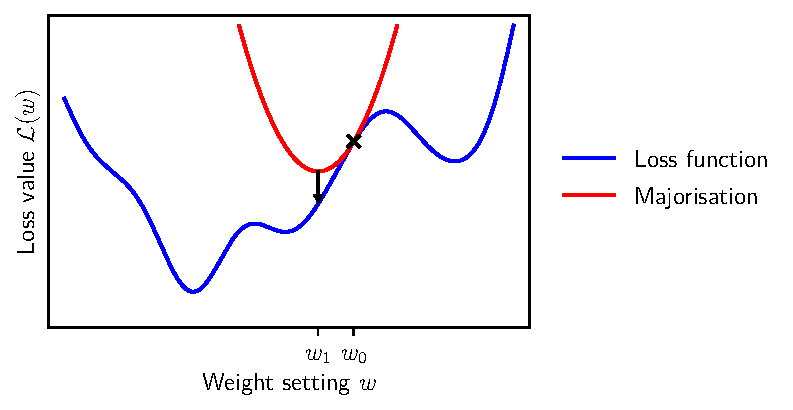
\includegraphics{figures/maj-min.pdf}
    \caption[The majorise-minimise meta-algorithm]{The majorise-minimise meta-algorithm. The blue curve denotes a loss function that one would like to reduce, starting from a point $w_0$. The red curve denotes a \textit{majorisation} of the loss about $w_0$. Since the majorisation is both an upper bound to the loss that is also tangent at $w_0$, minimising the majorisation to obtain a new weight setting $w_1$ also reduces the original loss.}
    \label{fig:major-minor}
\end{figure}

\section{Instantiations of the meta-algorithm}
\label{sec:examples}

First-order optimisation methods minimise a majorisation of the first-order Taylor expansion of the loss function. They therefore rely on first-order \textit{gradient} information and do not have access to second-order \textit{Hessian} information. Examples include basic gradient descent and also \textit{mirror descent}.

Meanwhile, second-order optimisation methods minimise a majorisation of the second-order Taylor expansion of the loss function. Both first-order \textit{gradient} information as well as second-order \textit{Hessian} information are used. The hope is that including this extra information will lead to a more effective optimisation step. One example is the \textit{cubic-regularised} version of \textit{Newton's method}.

\subsection{First example: Gradient descent}

This subsection shows that gradient descent in its most basic form arises from the following majorisation of the first-order Taylor expansion of the loss:
\begin{equation}\label{eq:gd-major}
    \el(w+\Delta w) \leq \el(w) + \nabla_w \el(w)^\top \Delta w + \frac{\lambda}{2}\cdot \norm{\Delta w}_2^2,
\end{equation}
for some constant $\lambda>0$. This is a \textit{Euclidean} majorisation, since the Euclidean norm $\|\cdot\|_2$ characterises the realm of validity of the first-order Taylor expansion.

One must ask, for which loss functions is Inequality \ref{eq:gd-major} a valid majorisation? Here it helps to define the class of \textit{gradient-Lipschitz} loss functions.
\begin{definition}[Gradient-Lipschitz loss function] A loss function $\el:\R^d\to\R$ is \textit{gradient-Lipschitz} with constant $\lambda>0$ if:
\begin{equation}
    \norm{\nabla_w\el(w+\Delta w) - \nabla_w\el(w)}_2 \leq \lambda\cdot\norm{\Delta w}_2.
\end{equation}
\end{definition}

The following lemma shows that a gradient Lipschitz loss function is majorised according to Inequality \ref{eq:gd-major}.
\begin{lemma}[Gradient-Lipschitz Euclidean majorisation]\label{lem:g-lipsch-major} Given that a loss function $\el:\R^d \to \R$ is gradient-Lipschitz with constant $\lambda$, then the Euclidean majorisation (Inequality \ref{eq:gd-major}) holds.
\end{lemma}
\begin{proof} By the fundamental theorem of calculus, the Cauchy-Schwarz inequality and finally the gradient-Lipschitz property:
\begin{align*}
    &\el(w+\Delta w) - \left[\el(w) + \nabla_w \el(w)^\top \Delta w\right]\\ &\qquad\qquad= \int_0^1\diff{t}\; \left(\nabla_w \el(w+t\cdot \Delta w)-\nabla_w\el(w)\right)^\top\Delta w\\
    &\qquad\qquad\leq \int_0^1\diff{t}\; \norm{\nabla_w \el(w+t\cdot \Delta w)-\nabla_w\el(w)}_2\cdot\norm{\Delta w}_2\\
    &\qquad\qquad \leq \int_0^1\diff{t}\; t \cdot \lambda \cdot \norm{\Delta w}_2^2 = \frac{\lambda}{2}\cdot\norm{\Delta w}_2^2.
\end{align*}
The proof is completed by adding the first-order Taylor series to both sides.
\end{proof}

Finally, the following theorem shows that the gradient descent optimisation algorithm emerges via minimisation of the majorisation in Inequality \ref{eq:gd-major}.

\begin{theorem}[Gradient descent]\label{thm:gd} The following holds:
\begin{equation}
    \argmin_{\Delta w} \left[\el(w) + \nabla_w \el(w)^\top \Delta w + \frac{\lambda}{2} \cdot \norm{\Delta w}_2^2\right] = - \frac{1}{\lambda} \cdot \nabla_w \el(w).
\end{equation}
\end{theorem}
\begin{proof}
    Take the derivative of the minimand on the left-hand side with respect to $\Delta w$, set this derivative to zero, and solve for $\Delta w$.
\end{proof}

\subsection{Second example: Mirror descent}

The previous subsection showed that gradient descent in its most basic form arises from an intrinsically Euclidean majorisation of the loss. This subsection shows that a certain kind of \textit{non-Euclidean} majorisation leads to a variant of gradient descent known as \textit{mirror descent} \citep{nemirovsky_yudin_1983}.

The kind of non-Euclidean majorisation in question has a particular form: it assesses the error in the first-order Taylor expansion of a convex function:

\begin{definition}[Bregman divergence] Given a convex function $\psi:\mathcal{W} \to \R$, the \textit{Bregman divergence} $h_\psi:\mathcal{W}\times\mathcal{W} \to \R$ corresponding to $\psi$ is given by:
\begin{equation}
    h_\psi(w,w+\Delta w) \coloneqq \psi(w+\Delta w) - \left[\psi(w) + \nabla \psi(w)^\top \Delta w\right].
\end{equation}
\end{definition}
Note that by a basic property of convexity, $\psi(w+\Delta w)$ always lies above the tangent to $\psi$ at $w$, and therefore $h_\psi \geq 0$. Also, it is quick to check that $h_\psi$ satisfies the conditions of Definition \ref{def:majorisation} to be a valid majorisation of $\psi$.

One hopes to apply mirror descent in situations where the trust region of the loss function of interest $\el$ is well-modeled by $h_\psi$:

\begin{assumption}[Majorisation via Bregman divergence]\label{ass:bregman-major} For a loss function $\el: \mathcal{W} \to \R$ and a convex function $\psi:\mathcal{W} \to \R$, assume that:
\begin{equation}
    \el(w+\Delta w) \leq \el(w) + \nabla_w \el(w)^\top \Delta w + h_\psi(w,w+\Delta w).
\end{equation}
\end{assumption}
In words: the majorisation $h_\psi$ of convex function $\psi$ is assumed to also majorise the loss function $\el$. The reason that this assumption is interesting is that the corresponding majorise-minimise algorithm has a particularly elegant form:

\begin{proposition}[Mirror descent] Let perturbation $\Delta w_*$ denote the minimiser of the majorisation given in Assumption \ref{ass:bregman-major}:
\begin{equation}
    \Delta w_* \coloneqq \argmin_{\Delta w} \left[\el(w) + \nabla_w \el(w)^\top \Delta w + h_\psi(w,w+\Delta w) \right].
\end{equation}
Then $\Delta w_*$ satisfies the following first-order optimality condition:
\begin{equation}\label{eq:mirror-domain}
    \nabla \psi(w+\Delta w_*) = \nabla \psi(w) - \nabla_w\el(w).
\end{equation}
Furthermore, when $\nabla \psi$ is invertible, the optimal perturbation satisfies:
\begin{equation}\label{eq:mirror-back}
    w+\Delta w_* = \nabla \psi^{-1}\left[\nabla \psi(w) - \nabla_w\el(w)\right].
\end{equation}
\end{proposition}

Equation \ref{eq:mirror-domain} may be interpreted as a vanilla gradient descent update to optimisation variables that have been transformed by the map $\nabla\psi:\R^d\to\R^d$. So for the kind of non-Euclidean majorisation given in Assumption \ref{ass:bregman-major}, optimisation still admits a simple additive structure when viewed in the \textit{mirror domain} $\nabla \psi (\mathcal{W}) \coloneqq \{ \nabla \psi (w) : w\in\mathcal{W}\}$.

Mirror descent makes an important departure from the Euclidean structure of gradient descent by leveraging a particular kind of non-Euclidean majorisation given by a Bregman divergence (Assumption \ref{ass:bregman-major}). But there may be other means of constructing non-Euclidean majorisations. Non-Euclidean majorisations directly tailored to learning problems will be explored in Chapters \ref{chap:maj-min} and \ref{chap:nn-maj-min}.

\subsection{Third example: Cubic regularised Newton}

A first attempt toward building a second-order optimisation method is known as \textit{Newton's method}. Newton's method attempts to minimise the Taylor series expansion of the loss function truncated to second order:
\begin{equation}\label{eq:so-trunc}
    \Delta w^* = \argmin_{\Delta w} \left[\el(w) + \nabla_w \el(w)^\top \Delta w + \frac{1}{2}\cdot\Delta w^\top \nabla^2_w\el(w) \Delta w\right].
\end{equation}

Unfortunately, as was the case for minimising the first-order truncation (Equation \ref{eq:fo-trunc}), this procedure is generally not well-founded. For instance, if the Hessian $\nabla^2_w\el(w)$ has any negative eigenvalues, then the minimand appearing in Equation \ref{eq:so-trunc} can be made arbitrarily negative by selecting a $\Delta w$ in the corresponding negative eigenspace, with arbitrarily large magnitude.

Again, this issue may be solved by a majorisation. Just as Lemma \ref{lem:g-lipsch-major} showed that a gradient-Lipschitz loss function admits a quadratic majorisation of the first-order Taylor expansion, a Hessian-Lipschitz loss function admits a cubic majorisation of the second-order expansion. This insight leads to the \textit{cubic regularised} version of Newton's method due to \citet{Nesterov2006CubicRO}:
\begin{equation}
    \Delta w_* = \argmin_{\Delta w} \left[\el^{(2)}(w+\Delta w) + \frac{\lambda}{6}\cdot\norm{\Delta w}_2^3\right].
\end{equation}
\begin{table}[p]
    \centering
    \def\arraystretch{2}
    \begin{tabular*}{\textwidth}{l @{\extracolsep{\fill}} cc}
    \textbf{Optimiser} & \textbf{Truncation order, $\mathbf{k}$} &  \textbf{Majorisation, $\mathbf{h}$} \\
    gradient descent & $k=1$ & $\displaystyle \frac{\lambda}{2} \cdot \norm{\Delta w}_2^2$ \\
    mirror descent & $k=1$ & $\displaystyle h_\psi(w,w+\Delta w)$\\
    cubic regularised Newton & $k=2$ & $\displaystyle \frac{\lambda}{6}\cdot\norm{\Delta w}_2^3$ \\
    \end{tabular*}
    \vspace{4ex}
    \caption[Optimisation methods and their corresponding majorisations]{Optimisation methods and their corresponding majorisations. Each optimiser perturbs a weight vector $w\mapsto w+\Delta w_*$ where the perturbation $\Delta w_*$ is selected by solving $\Delta w_* = \argmin_{\Delta w}[\el^{(k)}(w+\Delta w) + h(w,\Delta w)]$. In this expression, $\el^{(k)}(w+\Delta w)$ refers to the Taylor series expansion of $\el(w+\Delta w)$ in perturbation $\Delta w$ truncated to $k$th order.}
    \label{tab:trust}
\end{table}

The authors show how to solve this optimisation sub-problem, and provide some global convergence results for this method in certain settings.

\clearpage

\section{Trade-off between computation and fidelity}

This chapter has presented derivations of various optimisation methods, summarised in Table \ref{tab:trust}. The derivations work by majorising a truncated Taylor expansion in weight perturbations, and then minimising this majorisation. This process is formally described by Equation \ref{eq:minor} and illustrated in Figure \ref{fig:major-minor}.

What has not been discussed is the computational complexity of this procedure. In general, there is a trade-off between the fidelity of any particular majorisation, and the computational cost of its evaluation. For instance, majorising a higher-order Taylor expansion may lead to a tighter perturbation bound with a larger region of validity, allowing each optimisation step to make more progress. But one needs to ask if this larger per-step improvement is worth the extra computational overhead of evaluating a higher-order perturbation bound.

A good case in point is first-order versus second-order methods. While the per-step improvement of a second-order method may well exceed that of a first-order method, the per-step cost of the second-order method may be prohibitively expensive. On a $d$-dimensional weight space, $\mathcal{W}=\R^d$:
\begin{enumerate}
    \item The Hessian matrix $\nabla_w^2\el(w)\in\R^{d\times d}$ requires $\mathcal{O}(d^2)$ memory to store.
    \item The gradient vector $\nabla_w\el(w)\in\R^{d}$ requires $\mathcal{O}(d)$ memory to store.
\end{enumerate}

So first-order methods may be preferable on high-dimensional weight spaces.

\printbibliography[heading=subbibliography]
\end{refsection}

